% Options for packages loaded elsewhere
\PassOptionsToPackage{unicode}{hyperref}
\PassOptionsToPackage{hyphens}{url}
\PassOptionsToPackage{dvipsnames,svgnames,x11names}{xcolor}
%
\documentclass[
  letterpaper,
  DIV=11,
  numbers=noendperiod]{scrartcl}

\usepackage{amsmath,amssymb}
\usepackage{iftex}
\ifPDFTeX
  \usepackage[T1]{fontenc}
  \usepackage[utf8]{inputenc}
  \usepackage{textcomp} % provide euro and other symbols
\else % if luatex or xetex
  \usepackage{unicode-math}
  \defaultfontfeatures{Scale=MatchLowercase}
  \defaultfontfeatures[\rmfamily]{Ligatures=TeX,Scale=1}
\fi
\usepackage{lmodern}
\ifPDFTeX\else  
    % xetex/luatex font selection
\fi
% Use upquote if available, for straight quotes in verbatim environments
\IfFileExists{upquote.sty}{\usepackage{upquote}}{}
\IfFileExists{microtype.sty}{% use microtype if available
  \usepackage[]{microtype}
  \UseMicrotypeSet[protrusion]{basicmath} % disable protrusion for tt fonts
}{}
\makeatletter
\@ifundefined{KOMAClassName}{% if non-KOMA class
  \IfFileExists{parskip.sty}{%
    \usepackage{parskip}
  }{% else
    \setlength{\parindent}{0pt}
    \setlength{\parskip}{6pt plus 2pt minus 1pt}}
}{% if KOMA class
  \KOMAoptions{parskip=half}}
\makeatother
\usepackage{xcolor}
\setlength{\emergencystretch}{3em} % prevent overfull lines
\setcounter{secnumdepth}{5}
% Make \paragraph and \subparagraph free-standing
\makeatletter
\ifx\paragraph\undefined\else
  \let\oldparagraph\paragraph
  \renewcommand{\paragraph}{
    \@ifstar
      \xxxParagraphStar
      \xxxParagraphNoStar
  }
  \newcommand{\xxxParagraphStar}[1]{\oldparagraph*{#1}\mbox{}}
  \newcommand{\xxxParagraphNoStar}[1]{\oldparagraph{#1}\mbox{}}
\fi
\ifx\subparagraph\undefined\else
  \let\oldsubparagraph\subparagraph
  \renewcommand{\subparagraph}{
    \@ifstar
      \xxxSubParagraphStar
      \xxxSubParagraphNoStar
  }
  \newcommand{\xxxSubParagraphStar}[1]{\oldsubparagraph*{#1}\mbox{}}
  \newcommand{\xxxSubParagraphNoStar}[1]{\oldsubparagraph{#1}\mbox{}}
\fi
\makeatother

\usepackage{color}
\usepackage{fancyvrb}
\newcommand{\VerbBar}{|}
\newcommand{\VERB}{\Verb[commandchars=\\\{\}]}
\DefineVerbatimEnvironment{Highlighting}{Verbatim}{commandchars=\\\{\}}
% Add ',fontsize=\small' for more characters per line
\usepackage{framed}
\definecolor{shadecolor}{RGB}{241,243,245}
\newenvironment{Shaded}{\begin{snugshade}}{\end{snugshade}}
\newcommand{\AlertTok}[1]{\textcolor[rgb]{0.68,0.00,0.00}{#1}}
\newcommand{\AnnotationTok}[1]{\textcolor[rgb]{0.37,0.37,0.37}{#1}}
\newcommand{\AttributeTok}[1]{\textcolor[rgb]{0.40,0.45,0.13}{#1}}
\newcommand{\BaseNTok}[1]{\textcolor[rgb]{0.68,0.00,0.00}{#1}}
\newcommand{\BuiltInTok}[1]{\textcolor[rgb]{0.00,0.23,0.31}{#1}}
\newcommand{\CharTok}[1]{\textcolor[rgb]{0.13,0.47,0.30}{#1}}
\newcommand{\CommentTok}[1]{\textcolor[rgb]{0.37,0.37,0.37}{#1}}
\newcommand{\CommentVarTok}[1]{\textcolor[rgb]{0.37,0.37,0.37}{\textit{#1}}}
\newcommand{\ConstantTok}[1]{\textcolor[rgb]{0.56,0.35,0.01}{#1}}
\newcommand{\ControlFlowTok}[1]{\textcolor[rgb]{0.00,0.23,0.31}{\textbf{#1}}}
\newcommand{\DataTypeTok}[1]{\textcolor[rgb]{0.68,0.00,0.00}{#1}}
\newcommand{\DecValTok}[1]{\textcolor[rgb]{0.68,0.00,0.00}{#1}}
\newcommand{\DocumentationTok}[1]{\textcolor[rgb]{0.37,0.37,0.37}{\textit{#1}}}
\newcommand{\ErrorTok}[1]{\textcolor[rgb]{0.68,0.00,0.00}{#1}}
\newcommand{\ExtensionTok}[1]{\textcolor[rgb]{0.00,0.23,0.31}{#1}}
\newcommand{\FloatTok}[1]{\textcolor[rgb]{0.68,0.00,0.00}{#1}}
\newcommand{\FunctionTok}[1]{\textcolor[rgb]{0.28,0.35,0.67}{#1}}
\newcommand{\ImportTok}[1]{\textcolor[rgb]{0.00,0.46,0.62}{#1}}
\newcommand{\InformationTok}[1]{\textcolor[rgb]{0.37,0.37,0.37}{#1}}
\newcommand{\KeywordTok}[1]{\textcolor[rgb]{0.00,0.23,0.31}{\textbf{#1}}}
\newcommand{\NormalTok}[1]{\textcolor[rgb]{0.00,0.23,0.31}{#1}}
\newcommand{\OperatorTok}[1]{\textcolor[rgb]{0.37,0.37,0.37}{#1}}
\newcommand{\OtherTok}[1]{\textcolor[rgb]{0.00,0.23,0.31}{#1}}
\newcommand{\PreprocessorTok}[1]{\textcolor[rgb]{0.68,0.00,0.00}{#1}}
\newcommand{\RegionMarkerTok}[1]{\textcolor[rgb]{0.00,0.23,0.31}{#1}}
\newcommand{\SpecialCharTok}[1]{\textcolor[rgb]{0.37,0.37,0.37}{#1}}
\newcommand{\SpecialStringTok}[1]{\textcolor[rgb]{0.13,0.47,0.30}{#1}}
\newcommand{\StringTok}[1]{\textcolor[rgb]{0.13,0.47,0.30}{#1}}
\newcommand{\VariableTok}[1]{\textcolor[rgb]{0.07,0.07,0.07}{#1}}
\newcommand{\VerbatimStringTok}[1]{\textcolor[rgb]{0.13,0.47,0.30}{#1}}
\newcommand{\WarningTok}[1]{\textcolor[rgb]{0.37,0.37,0.37}{\textit{#1}}}

\providecommand{\tightlist}{%
  \setlength{\itemsep}{0pt}\setlength{\parskip}{0pt}}\usepackage{longtable,booktabs,array}
\usepackage{calc} % for calculating minipage widths
% Correct order of tables after \paragraph or \subparagraph
\usepackage{etoolbox}
\makeatletter
\patchcmd\longtable{\par}{\if@noskipsec\mbox{}\fi\par}{}{}
\makeatother
% Allow footnotes in longtable head/foot
\IfFileExists{footnotehyper.sty}{\usepackage{footnotehyper}}{\usepackage{footnote}}
\makesavenoteenv{longtable}
\usepackage{graphicx}
\makeatletter
\newsavebox\pandoc@box
\newcommand*\pandocbounded[1]{% scales image to fit in text height/width
  \sbox\pandoc@box{#1}%
  \Gscale@div\@tempa{\textheight}{\dimexpr\ht\pandoc@box+\dp\pandoc@box\relax}%
  \Gscale@div\@tempb{\linewidth}{\wd\pandoc@box}%
  \ifdim\@tempb\p@<\@tempa\p@\let\@tempa\@tempb\fi% select the smaller of both
  \ifdim\@tempa\p@<\p@\scalebox{\@tempa}{\usebox\pandoc@box}%
  \else\usebox{\pandoc@box}%
  \fi%
}
% Set default figure placement to htbp
\def\fps@figure{htbp}
\makeatother

\KOMAoption{captions}{tableheading}
\makeatletter
\@ifpackageloaded{caption}{}{\usepackage{caption}}
\AtBeginDocument{%
\ifdefined\contentsname
  \renewcommand*\contentsname{Table of contents}
\else
  \newcommand\contentsname{Table of contents}
\fi
\ifdefined\listfigurename
  \renewcommand*\listfigurename{List of Figures}
\else
  \newcommand\listfigurename{List of Figures}
\fi
\ifdefined\listtablename
  \renewcommand*\listtablename{List of Tables}
\else
  \newcommand\listtablename{List of Tables}
\fi
\ifdefined\figurename
  \renewcommand*\figurename{Figure}
\else
  \newcommand\figurename{Figure}
\fi
\ifdefined\tablename
  \renewcommand*\tablename{Table}
\else
  \newcommand\tablename{Table}
\fi
}
\@ifpackageloaded{float}{}{\usepackage{float}}
\floatstyle{ruled}
\@ifundefined{c@chapter}{\newfloat{codelisting}{h}{lop}}{\newfloat{codelisting}{h}{lop}[chapter]}
\floatname{codelisting}{Listing}
\newcommand*\listoflistings{\listof{codelisting}{List of Listings}}
\makeatother
\makeatletter
\makeatother
\makeatletter
\@ifpackageloaded{caption}{}{\usepackage{caption}}
\@ifpackageloaded{subcaption}{}{\usepackage{subcaption}}
\makeatother

\usepackage{bookmark}

\IfFileExists{xurl.sty}{\usepackage{xurl}}{} % add URL line breaks if available
\urlstyle{same} % disable monospaced font for URLs
\hypersetup{
  pdftitle={3. Übungsblatt (Ereignisdatenanalyse)},
  pdfauthor={Daria Tisch},
  colorlinks=true,
  linkcolor={blue},
  filecolor={Maroon},
  citecolor={Blue},
  urlcolor={Blue},
  pdfcreator={LaTeX via pandoc}}


\title{3. Übungsblatt (Ereignisdatenanalyse)}
\author{Daria Tisch}
\date{}

\begin{document}
\maketitle


\section{Organisation}\label{organisation}

\subsection{Arbeitsverzeichnis
festsetzen}\label{arbeitsverzeichnis-festsetzen}

\begin{Shaded}
\begin{Highlighting}[]
\CommentTok{\# set working directory}
\FunctionTok{setwd}\NormalTok{(}\StringTok{"C:/Users/ti/Local/seafile/main/teaching/2024\_wuppertal/studis/uebungen"}\NormalTok{)}
\end{Highlighting}
\end{Shaded}

\subsection{Packages installieren und
laden}\label{packages-installieren-und-laden}

\begin{Shaded}
\begin{Highlighting}[]
\CommentTok{\# Packages}
\NormalTok{pkgs }\OtherTok{\textless{}{-}} \FunctionTok{c}\NormalTok{(}
  \StringTok{"tidyverse"}\NormalTok{,}
  \StringTok{"sjPlot"}\NormalTok{, }\CommentTok{\# nice html tables}
  \StringTok{"survival"}\NormalTok{, }\CommentTok{\# survival analysis}
  \StringTok{"ggsurvfit"} \CommentTok{\# flexible time{-}to{-}event figures}
\NormalTok{) }

\DocumentationTok{\#\# Install uninstalled packages}
\FunctionTok{lapply}\NormalTok{(pkgs[}\SpecialCharTok{!}\NormalTok{(pkgs }\SpecialCharTok{\%in\%} \FunctionTok{installed.packages}\NormalTok{())], install.packages)}

\DocumentationTok{\#\# Load all packages to library}
\FunctionTok{lapply}\NormalTok{(pkgs, library, }\AttributeTok{character.only =} \ConstantTok{TRUE}\NormalTok{)}
\end{Highlighting}
\end{Shaded}

\subsection{Daten einlesen}\label{daten-einlesen}

Wir arbeiten mit einem Datensatz, der Teil des R-Pakets \{survival\}
ist. Bitte lasse Dir alle Datensätze des Pakets anzeigen und speichere
den Datensatz lung als \emph{df}.

Datensätze, die im Package survival enthalten sind, anzeigen:

\begin{Shaded}
\begin{Highlighting}[]
\FunctionTok{data}\NormalTok{(}\AttributeTok{package =} \StringTok{"survival"}\NormalTok{)}
\end{Highlighting}
\end{Shaded}

\emph{lung} Datensatz als \emph{df} speichern:

\begin{Shaded}
\begin{Highlighting}[]
\CommentTok{\# Lungenkrebsdatensatz als df speichern }
\NormalTok{df }\OtherTok{=}\NormalTok{ lung}
\end{Highlighting}
\end{Shaded}

Schaue Dir nun die Beschreibung des Datensatzes an:

\begin{Shaded}
\begin{Highlighting}[]
\NormalTok{?lung}
\end{Highlighting}
\end{Shaded}

\begin{verbatim}
starte den http Server für die Hilfe fertig
\end{verbatim}

Der Datensatz enthält also Informationen zu PatientInnen der North
Central Cancer Treatment Group.

\section{Datenaufbereitung}\label{datenaufbereitung}

In dieser Übung möchten wir untersuchen, ob es Unterschiede zwischen
Männern und Frauen in der Überlebenszeit bei Lungenkrebs gibt.

Wir brauchen für unsere Analyse daher die folgenden 3 Variablen:

\begin{itemize}
\tightlist
\item
  dead (0: lebend, 1: tot)
\item
  female (0: männlich, 1: weiblich)
\item
  time (Tage)
\end{itemize}

Bitte suche diese heraus oder erstelle sie.

\begin{Shaded}
\begin{Highlighting}[]
\NormalTok{df }\OtherTok{\textless{}{-}}\NormalTok{ df }\SpecialCharTok{\%\textgreater{}\%} 
  \FunctionTok{mutate}\NormalTok{(}
    \AttributeTok{dead =} \FunctionTok{recode}\NormalTok{(status, }\StringTok{\textasciigrave{}}\AttributeTok{1}\StringTok{\textasciigrave{}} \OtherTok{=} \DecValTok{0}\NormalTok{, }\StringTok{\textasciigrave{}}\AttributeTok{2}\StringTok{\textasciigrave{}} \OtherTok{=} \DecValTok{1}\NormalTok{),}
    \AttributeTok{female =} \FunctionTok{recode}\NormalTok{(sex, }\StringTok{\textasciigrave{}}\AttributeTok{1}\StringTok{\textasciigrave{}} \OtherTok{=} \DecValTok{0}\NormalTok{, }\StringTok{\textasciigrave{}}\AttributeTok{2}\StringTok{\textasciigrave{}} \OtherTok{=} \DecValTok{1}\NormalTok{)}
\NormalTok{  )}
\end{Highlighting}
\end{Shaded}

\section{Datenexploration}\label{datenexploration}

\subsection{Anzahl Beobachtungen}\label{anzahl-beobachtungen}

Wie viele Personen sind in dem Datensatz?

\begin{Shaded}
\begin{Highlighting}[]
\FunctionTok{length}\NormalTok{(df}\SpecialCharTok{$}\NormalTok{dead)}
\end{Highlighting}
\end{Shaded}

\begin{verbatim}
[1] 228
\end{verbatim}

\begin{Shaded}
\begin{Highlighting}[]
\FunctionTok{nrow}\NormalTok{(lung)}
\end{Highlighting}
\end{Shaded}

\begin{verbatim}
[1] 228
\end{verbatim}

\subsection{Anzahl Frauen und Männer}\label{anzahl-frauen-und-muxe4nner}

Wie viele Frauen und Männer sind jewils in dem Datensatz?

\begin{Shaded}
\begin{Highlighting}[]
\FunctionTok{table}\NormalTok{(df}\SpecialCharTok{$}\NormalTok{female)}
\end{Highlighting}
\end{Shaded}

\begin{verbatim}

  0   1 
138  90 
\end{verbatim}

\subsection{Anzahl Personden, die im Beobachtungszeitraum gestorben
sind}\label{anzahl-personden-die-im-beobachtungszeitraum-gestorben-sind}

Wie viele Personen sind im Beobachtungszeitraum gestorben?

\begin{Shaded}
\begin{Highlighting}[]
\FunctionTok{table}\NormalTok{(df}\SpecialCharTok{$}\NormalTok{dead)}
\end{Highlighting}
\end{Shaded}

\begin{verbatim}

  0   1 
 63 165 
\end{verbatim}

\subsection{Kreuztabelle Geschlecht und
Überleben}\label{kreuztabelle-geschlecht-und-uxfcberleben}

Wie viel Prozent der Frauen und wie viel Prozent der Männer sind im
Beobachtungszeitraum gestorben?

\begin{Shaded}
\begin{Highlighting}[]
\NormalTok{df }\SpecialCharTok{\%\textgreater{}\%}
  \FunctionTok{group\_by}\NormalTok{(female) }\SpecialCharTok{\%\textgreater{}\%}
  \FunctionTok{summarise}\NormalTok{(}
    \AttributeTok{total =} \FunctionTok{n}\NormalTok{(),                           }\CommentTok{\# Gesamtanzahl je Geschlecht}
    \AttributeTok{deaths =} \FunctionTok{sum}\NormalTok{(dead }\SpecialCharTok{==} \DecValTok{1}\NormalTok{),             }\CommentTok{\# Anzahl der gestorbenen Personen}
    \AttributeTok{percent\_deaths =}\NormalTok{ (deaths }\SpecialCharTok{/}\NormalTok{ total) }\SpecialCharTok{*} \DecValTok{100}  \CommentTok{\# Prozentsatz der Gestorbenen}
\NormalTok{  ) }\SpecialCharTok{\%\textgreater{}\%}
  \FunctionTok{arrange}\NormalTok{(female) }
\end{Highlighting}
\end{Shaded}

\begin{verbatim}
# A tibble: 2 x 4
  female total deaths percent_deaths
   <dbl> <int>  <int>          <dbl>
1      0   138    112           81.2
2      1    90     53           58.9
\end{verbatim}

\section{Ereignisdatenanalyse}\label{ereignisdatenanalyse}

\subsection{Zensierung}\label{zensierung}

Wie viele rechtszensierte und wie viele linkszentrierte Beobachtungen
liegen vor?

\begin{Shaded}
\begin{Highlighting}[]
\FunctionTok{table}\NormalTok{(df}\SpecialCharTok{$}\NormalTok{dead)}
\end{Highlighting}
\end{Shaded}

\begin{verbatim}

  0   1 
 63 165 
\end{verbatim}

\subsection{Erste 10 Fälle}\label{erste-10-fuxe4lle}

Schauen wir uns die ersten 10 Fälle des Datensatzes an. Was bedeutet das
+ hinter einer Zahl?

\begin{Shaded}
\begin{Highlighting}[]
\FunctionTok{Surv}\NormalTok{(df}\SpecialCharTok{$}\NormalTok{time, df}\SpecialCharTok{$}\NormalTok{dead)[}\DecValTok{1}\SpecialCharTok{:}\DecValTok{10}\NormalTok{]}
\end{Highlighting}
\end{Shaded}

\begin{verbatim}
 [1]  306   455  1010+  210   883  1022+  310   361   218   166 
\end{verbatim}

Das + bedeutet, dass es sich um rechtszensierte Fälle handelt. Diese
Personen leben zum Ende des Beobachtungszeintraums noch.

Was ist wohl der Nullpunkt der Zeitvariable \emph{time}?

\subsection{Kaplan-Meier-Kurve}\label{kaplan-meier-kurve}

Erstelle eine Kaplan-Meier-Kurve.

\begin{Shaded}
\begin{Highlighting}[]
\FunctionTok{survfit2}\NormalTok{(}\FunctionTok{Surv}\NormalTok{(time, dead) }\SpecialCharTok{\textasciitilde{}} \DecValTok{1}\NormalTok{, }\AttributeTok{data =}\NormalTok{ df) }\SpecialCharTok{\%\textgreater{}\%} 
  \FunctionTok{ggsurvfit}\NormalTok{() }\SpecialCharTok{+}
  \FunctionTok{labs}\NormalTok{(}
    \AttributeTok{x =} \StringTok{"Tage"}\NormalTok{,}
    \AttributeTok{y =} \StringTok{"Überlebenswahrscheinlichkeit"}
\NormalTok{  )}
\end{Highlighting}
\end{Shaded}

\pandocbounded{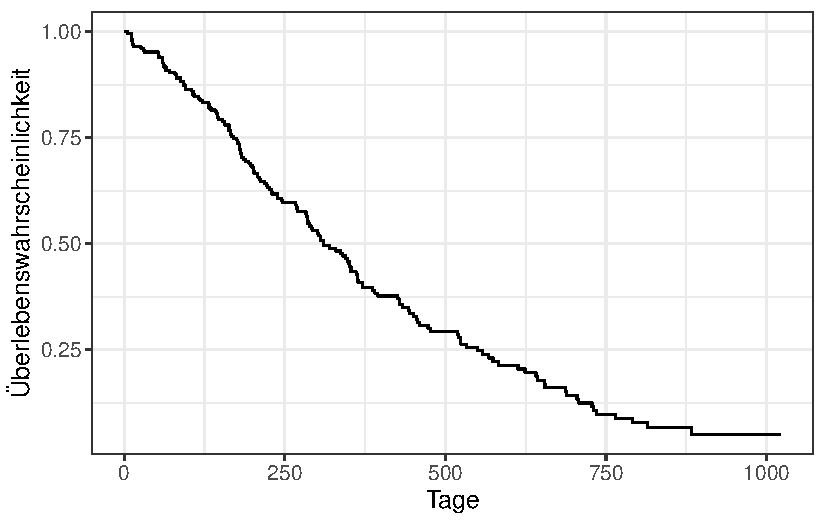
\includegraphics[keepaspectratio]{3_uebungsblatt_files/figure-pdf/unnamed-chunk-13-1.pdf}}

\subsection{Kaplan-Meier-Kurve mit KI}\label{kaplan-meier-kurve-mit-ki}

Nun ergänze die Kurve mit einem Konfidenzintervall.

\begin{Shaded}
\begin{Highlighting}[]
\FunctionTok{survfit2}\NormalTok{(}\FunctionTok{Surv}\NormalTok{(time, dead) }\SpecialCharTok{\textasciitilde{}} \DecValTok{1}\NormalTok{, }\AttributeTok{data =}\NormalTok{ df) }\SpecialCharTok{\%\textgreater{}\%} 
  \FunctionTok{ggsurvfit}\NormalTok{() }\SpecialCharTok{+}
  \FunctionTok{labs}\NormalTok{(}
    \AttributeTok{x =} \StringTok{"Tage"}\NormalTok{,}
    \AttributeTok{y =} \StringTok{"Überlebenswahrscheinlichkeit"}
\NormalTok{  )}\SpecialCharTok{+} 
  \FunctionTok{add\_confidence\_interval}\NormalTok{()}
\end{Highlighting}
\end{Shaded}

\pandocbounded{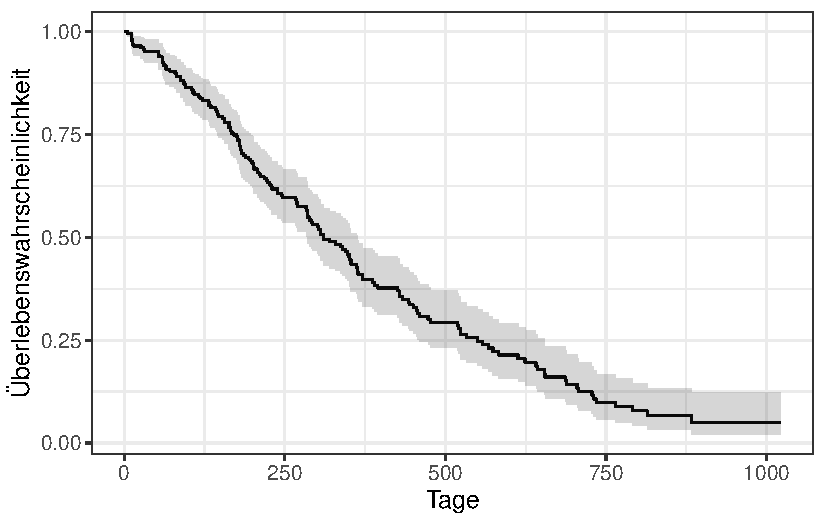
\includegraphics[keepaspectratio]{3_uebungsblatt_files/figure-pdf/unnamed-chunk-14-1.pdf}}

\subsection{Kaplan-Meier-Kurve mit Ki und
Risikotabelle}\label{kaplan-meier-kurve-mit-ki-und-risikotabelle}

Und nun füge bitte noch eine Risikotabelle hinzu.

\begin{Shaded}
\begin{Highlighting}[]
\FunctionTok{survfit2}\NormalTok{(}\FunctionTok{Surv}\NormalTok{(time, dead) }\SpecialCharTok{\textasciitilde{}} \DecValTok{1}\NormalTok{, }\AttributeTok{data =}\NormalTok{ df) }\SpecialCharTok{\%\textgreater{}\%} 
  \FunctionTok{ggsurvfit}\NormalTok{() }\SpecialCharTok{+}
  \FunctionTok{labs}\NormalTok{(}
    \AttributeTok{x =} \StringTok{"Tage"}\NormalTok{,}
    \AttributeTok{y =} \StringTok{"Überlebenswahrscheinlichkeit"}
\NormalTok{  )}\SpecialCharTok{+} 
  \FunctionTok{add\_confidence\_interval}\NormalTok{() }\SpecialCharTok{+}
  \FunctionTok{add\_risktable}\NormalTok{()}
\end{Highlighting}
\end{Shaded}

\pandocbounded{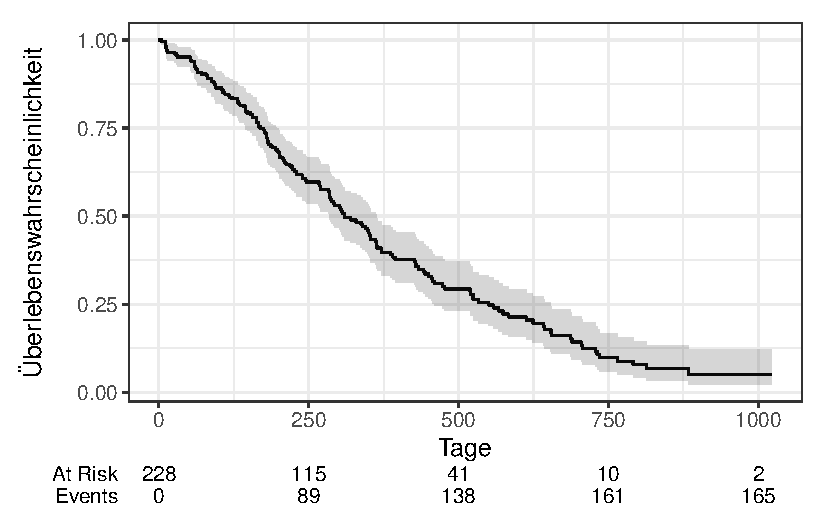
\includegraphics[keepaspectratio]{3_uebungsblatt_files/figure-pdf/unnamed-chunk-15-1.pdf}}

Wie viele Personen leben nach 500 Tagen noch?

\subsection{Schätzung der Überlebensrate nach einem
Jahr}\label{schuxe4tzung-der-uxfcberlebensrate-nach-einem-jahr}

\begin{Shaded}
\begin{Highlighting}[]
\FunctionTok{summary}\NormalTok{(}\FunctionTok{survfit}\NormalTok{(}\FunctionTok{Surv}\NormalTok{(time, dead) }\SpecialCharTok{\textasciitilde{}} \DecValTok{1}\NormalTok{, }\AttributeTok{data =}\NormalTok{ df), }\AttributeTok{times =} \DecValTok{365}\NormalTok{)}
\end{Highlighting}
\end{Shaded}

\begin{verbatim}
Call: survfit(formula = Surv(time, dead) ~ 1, data = df)

 time n.risk n.event survival std.err lower 95% CI upper 95% CI
  365     65     121    0.409  0.0358        0.345        0.486
\end{verbatim}

Wir stellen fest, dass die 1-Jahres-Überlebenswahrscheinlichkeit in
dieser Studie 41\% beträgt.

\section{Überlebenszeit im Median}\label{uxfcberlebenszeit-im-median}

Wie viele Tage übleben die PatientInnen im Median?

\begin{Shaded}
\begin{Highlighting}[]
\FunctionTok{survfit}\NormalTok{(}\FunctionTok{Surv}\NormalTok{(time, dead) }\SpecialCharTok{\textasciitilde{}} \DecValTok{1}\NormalTok{, }\AttributeTok{data =}\NormalTok{ df)}
\end{Highlighting}
\end{Shaded}

\begin{verbatim}
Call: survfit(formula = Surv(time, dead) ~ 1, data = df)

       n events median 0.95LCL 0.95UCL
[1,] 228    165    310     285     363
\end{verbatim}

\section{Kaplan-Meier-Kurve nach
Geschlecht}\label{kaplan-meier-kurve-nach-geschlecht}

Nun möchten wir die Geschlechterunterschiede in der
Überlebenswahrscheinlichkeit über die Zeit graphisch untersuchen.

\begin{Shaded}
\begin{Highlighting}[]
\FunctionTok{survfit2}\NormalTok{(}\FunctionTok{Surv}\NormalTok{(time, dead) }\SpecialCharTok{\textasciitilde{}}\NormalTok{ female, }\AttributeTok{data =}\NormalTok{ df) }\SpecialCharTok{\%\textgreater{}\%} 
  \FunctionTok{ggsurvfit}\NormalTok{() }\SpecialCharTok{+}
  \FunctionTok{labs}\NormalTok{(}
    \AttributeTok{x =} \StringTok{"Tage"}\NormalTok{,}
    \AttributeTok{y =} \StringTok{"Überlebenswahrscheinlichkeit"}\NormalTok{,}
    \AttributeTok{color =} \StringTok{"Geschlecht"}
\NormalTok{  )}\SpecialCharTok{+} 
  \FunctionTok{add\_confidence\_interval}\NormalTok{() }\SpecialCharTok{+}
  \FunctionTok{add\_risktable}\NormalTok{() }\SpecialCharTok{+} 
 \FunctionTok{scale\_color\_manual}\NormalTok{(}\AttributeTok{values =} \FunctionTok{c}\NormalTok{(}\StringTok{\textquotesingle{}darkblue\textquotesingle{}}\NormalTok{, }\StringTok{\textquotesingle{}darkred\textquotesingle{}}\NormalTok{),  }\AttributeTok{labels =} \FunctionTok{c}\NormalTok{(}\StringTok{"Männer"}\NormalTok{, }\StringTok{"Frauen"}\NormalTok{) ) }\SpecialCharTok{+}
  \FunctionTok{scale\_fill\_manual}\NormalTok{(}\AttributeTok{values =} \FunctionTok{c}\NormalTok{(}\StringTok{\textquotesingle{}darkblue\textquotesingle{}}\NormalTok{, }\StringTok{\textquotesingle{}darkred\textquotesingle{}}\NormalTok{),  }\AttributeTok{labels =} \FunctionTok{c}\NormalTok{(}\StringTok{"Männer"}\NormalTok{, }\StringTok{"Frauen"}\NormalTok{) ) }\SpecialCharTok{+}
  \FunctionTok{theme\_minimal}\NormalTok{() }\SpecialCharTok{+} \FunctionTok{guides}\NormalTok{(}\AttributeTok{fill =} \StringTok{"none"}\NormalTok{)}
\end{Highlighting}
\end{Shaded}

\pandocbounded{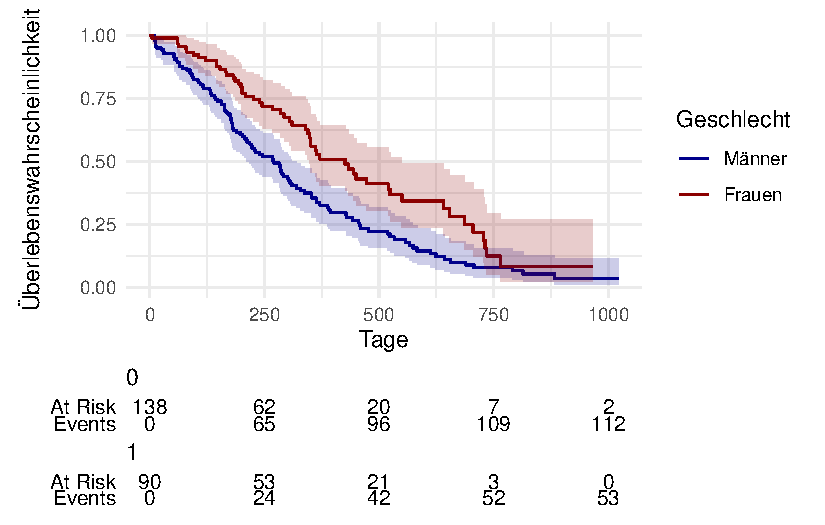
\includegraphics[keepaspectratio]{3_uebungsblatt_files/figure-pdf/unnamed-chunk-18-1.pdf}}

\section{Cox Proportional Hazards
Model}\label{cox-proportional-hazards-model}

Nun schätzen wir ein Cox Proportional Hazards Model. Gibt es
signifikante Geschlechterunterschiede? Ist die
Proportionalitätsannahme~erfüllt?

\begin{Shaded}
\begin{Highlighting}[]
\NormalTok{model1 }\OtherTok{=} \FunctionTok{coxph}\NormalTok{(}\FunctionTok{Surv}\NormalTok{(time, dead) }\SpecialCharTok{\textasciitilde{}}\NormalTok{ female, }\AttributeTok{data =}\NormalTok{ df)}
\FunctionTok{summary}\NormalTok{(model1)}
\end{Highlighting}
\end{Shaded}

\begin{verbatim}
Call:
coxph(formula = Surv(time, dead) ~ female, data = df)

  n= 228, number of events= 165 

          coef exp(coef) se(coef)      z Pr(>|z|)   
female -0.5310    0.5880   0.1672 -3.176  0.00149 **
---
Signif. codes:  0 '***' 0.001 '**' 0.01 '*' 0.05 '.' 0.1 ' ' 1

       exp(coef) exp(-coef) lower .95 upper .95
female     0.588      1.701    0.4237     0.816

Concordance= 0.579  (se = 0.021 )
Likelihood ratio test= 10.63  on 1 df,   p=0.001
Wald test            = 10.09  on 1 df,   p=0.001
Score (logrank) test = 10.33  on 1 df,   p=0.001
\end{verbatim}

\begin{Shaded}
\begin{Highlighting}[]
\FunctionTok{cox.zph}\NormalTok{(model1)}
\end{Highlighting}
\end{Shaded}

\begin{verbatim}
       chisq df     p
female  2.86  1 0.091
GLOBAL  2.86  1 0.091
\end{verbatim}

Erstelle eine Tabelle zur besseren Übersicht

\begin{Shaded}
\begin{Highlighting}[]
\FunctionTok{tab\_model}\NormalTok{(model1,}
          \AttributeTok{show.ci =} \ConstantTok{FALSE}\NormalTok{, }\AttributeTok{p.style =} \StringTok{"stars"}\NormalTok{,}
          \AttributeTok{string.se =} \StringTok{"se"}\NormalTok{, }\AttributeTok{string.est =} \StringTok{"HR"}\NormalTok{,}
          \AttributeTok{string.pred =} \StringTok{" "}\NormalTok{)}
\end{Highlighting}
\end{Shaded}

\begin{longtable}[]{@{}cc@{}}
\toprule\noalign{}
\endhead
\bottomrule\noalign{}
\endlastfoot
~ & Surv(time, dead) \\
& HR \\
female & 0.59 \textsuperscript{**} \\
Observations & 228 \\
R\textsuperscript{2} Nagelkerke & 0.046 \\
\multicolumn{2}{@{}r@{}}{%
* p\textless0.05~~~** p\textless0.01~~~*** p\textless0.001} \\
\end{longtable}

\subsection{\texorpdfstring{Interpretiere den Koeffizienten von
\emph{female}:}{Interpretiere den Koeffizienten von female:}}\label{interpretiere-den-koeffizienten-von-female}

Bei einem Cox-Regressionsmodell interessieren wir uns meist für die
Hazard Ratio (HR). Die HR stellt das Verhältnis der Risiken zwischen
zwei Gruppen zu einem bestimmten Zeitpunkt dar. Die HR wird als die
momentane Rate des Auftretens des interessierenden Ereignisses bei
denjenigen interpretiert, die noch ein Risiko für dieses Ereignis haben.
Die HR ist exp(β).

\begin{itemize}
\tightlist
\item
  HR \textless{} 1: verringertes Sterberisiko
\item
  HR \textgreater{} 1: erhöhtes Sterberisiko
\end{itemize}

HR = 0,59: Zu einem bestimmten Zeitpunkt sterben 0,59 mal so viele
Frauen wie Männer. Frauen haben in dieser Stichprobe ein deutlich
geringeres Sterberisiko als Männer.

\section{Render}\label{render}

Wandle dieses Dokument in ein PDF und ein HTML Dokument um.

\section{Weiterführende Literatur}\label{weiterfuxfchrende-literatur}

\begin{itemize}
\tightlist
\item
  \href{https://r4ds.had.co.nz/}{R for Data Science}
\item
  \url{https://www.emilyzabor.com/tutorials/survival_analysis_in_r_tutorial.html}
\end{itemize}




\end{document}
